\begin{figure}[!h]
	\begin{subfigure}{.5\textwidth}
		\centering
    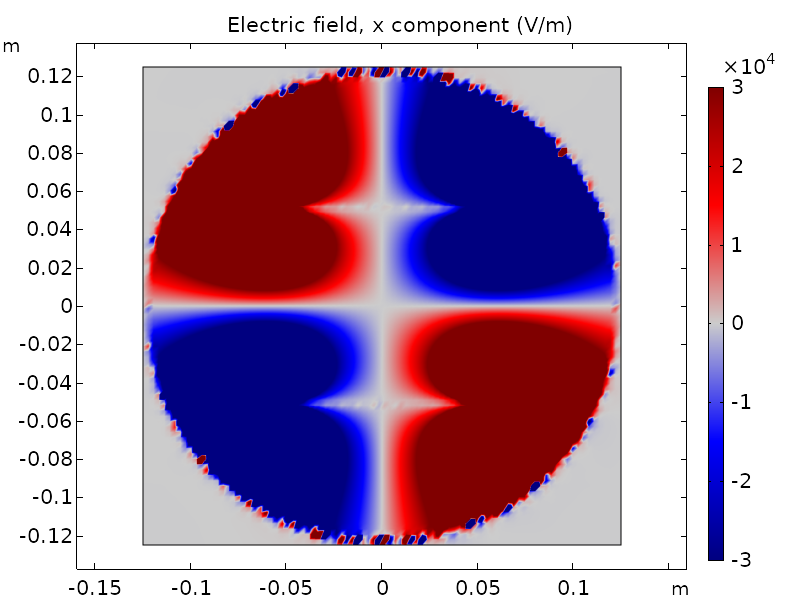
\includegraphics[width=\textwidth]{03_Prototype/figures/00_fig/fig012_BEMa.png}
		\caption{Asymmetric configuration.
			Readout is grounded while extracting electrode is at certain potential.}
		\label{fig:fconfig:asym_setup}
	\end{subfigure}\hfill
	\begin{subfigure}{.5\textwidth}
		\centering
    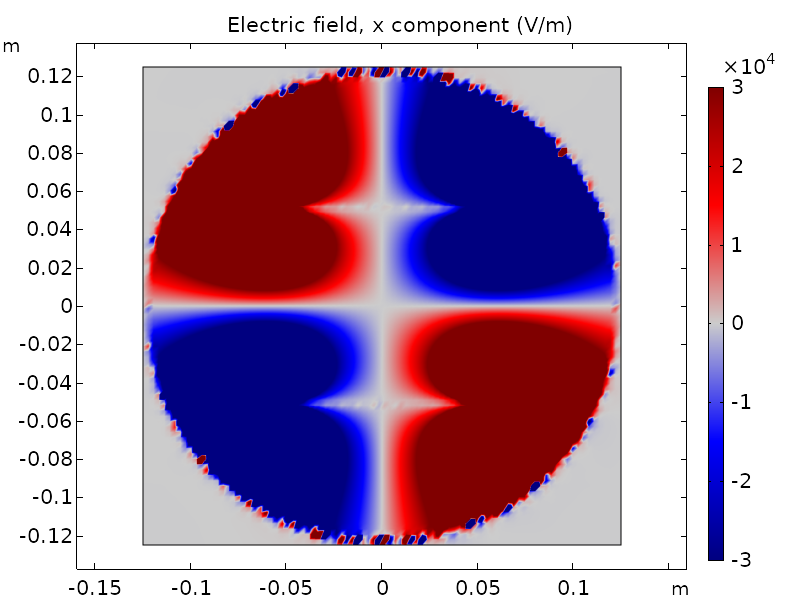
\includegraphics[width=\textwidth]{03_Prototype/figures/00_fig/fig012_BEMa.png}
		\caption{Symmetric configuration. Readout and extracting electrode are at opposite potential.}
		\label{fig:fconfig:sym_setup}
	\end{subfigure}
	\vskip\baselineskip
    \begin{subfigure}{.5\textwidth}
      \centering
      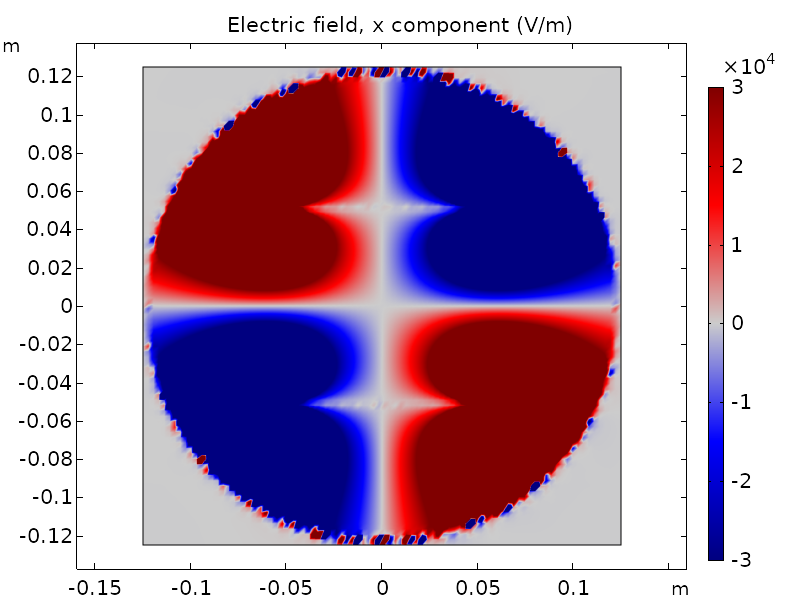
\includegraphics[width=\textwidth]{03_Prototype/figures/00_fig/fig012_BEMa.png}
      \caption{Electrical field in asymmetric configuration. There is no field corrections applied here.}
      \label{fig:fconfig:asym_field}
    \end{subfigure}\hfill
    \begin{subfigure}{.5\textwidth}
      \centering
      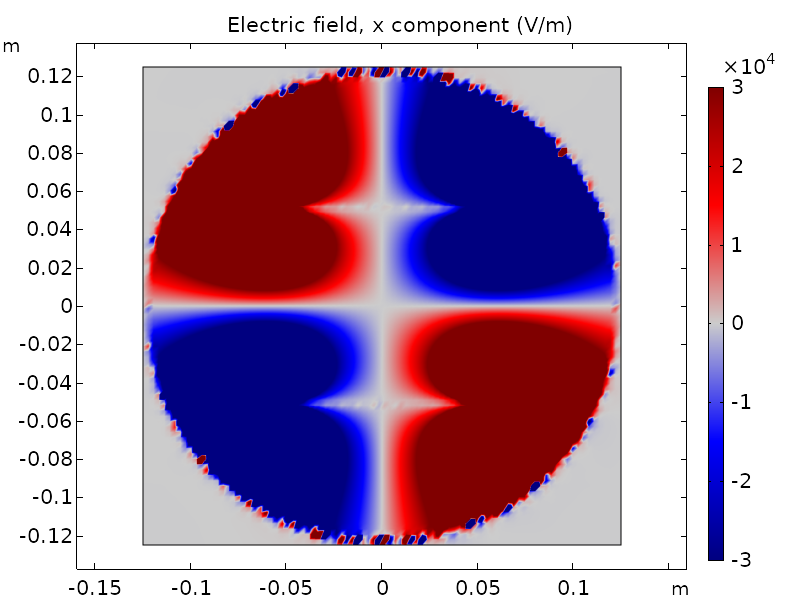
\includegraphics[width=\textwidth]{03_Prototype/figures/00_fig/fig012_BEMa.png}
      \caption{Electrical field in symmetric configuration. There is no field corrections applied here.}
      \label{fig:fconfig:sym_field}
    \end{subfigure}
    \caption [Asymmetric or symmetric configuration]
    {Asymmetric or symmetric configuration, MCPs allow both.}
    \label{fig:fconfig}
\end{figure}
